\documentclass{book}
% \usepackage[utf8]{inputenc}

\usepackage{amssymb,amsmath,amsfonts,eurosym,geometry,graphicx,caption,color,setspace,sectsty,footmisc,caption,array,hyperref,dsfont}

% \usepackage{indentfirst}	% make indent in first paragraph
\setlength\parindent{0pt}
\setlength{\parskip}{1em}
% \renewcommand{\baselinestretch}{1.5}

\usepackage{bm}
\usepackage{geometry}		% to make typesettings like margins
\usepackage{mathrsfs}
\usepackage{enumitem}

% \usepackage{natbib}			% to insert citations
\usepackage[natbib,authordate,noibid,backend=biber]{biblatex-chicago}
\addbibresource{../../reference-macwin.bib} % in Academic_Writings folder
% \addbibresource{C:/Users/Kaida/Dropbox/Academic_Writings/reference-win.bib}

\usepackage[table,xcdraw]{xcolor}			% extend the colors can be used

% \usepackage{bibentry}		% package used to insert full citation in body text
% replaced by \fullcite in biblatex

% \makeatletter 
% \renewcommand\BR@b@bibitem[2][]{\BR@bibitem[#1]{#2}\BR@c@bibitem{#2}}
% \makeatother
% \nobibliography*


\usepackage{setspace}		% set space for comment bullet

\usepackage{graphicx}		% to insert image
\graphicspath{ {images/} }

\usepackage[english]{babel}

\usepackage{tocbibind}		% to add toc and bib into table of content
\usepackage{bookmark}	% to separate the last chapter from previous ones

\usepackage{amsthm}
\makeatletter
\def\th@plain{%
  \thm@notefont{}% same as heading font
  \itshape % body font
}
\def\th@definition{%
  \thm@notefont{}% same as heading font
  \normalfont % body font
}


\theoremstyle{plain}
\newtheorem{thm}{Theorem}[section] % reset theorem numbering for each chapter
\theoremstyle{definition}
\newtheorem{defn}{Definition}[section] % definition numbers are dependent on theorem numbers
\newtheorem{exmp}{Example}[section] % same for example numbers
\newtheorem{lemma}[thm]{Lemma}
\newtheorem{prop}[thm]{Proposition}
\newtheorem{obs}{Observation}
\newtheorem{que}{Question}[section]
\newtheorem{assp}{Assumption}[section]

\newenvironment{myproof}
{\noindent\textit{Proof:}}{\hfill$\square$}

\newenvironment{answer}
{\noindent\textit{Answer:}}{\hfill$\square$}

% \citestyle{chicago}
\geometry{letterpaper, margin=0.75in}
% \setlength\parindent{0pt} % to cancel indent


% A list of new commands
\newcommand{\R}{\mathbb{R}}			% depends on the package amssymb
\newcommand{\F}{\mathcal{F}}
\newcommand{\myline}{\vspace{3mm} \hrule \vspace{4mm}}


\definecolor{battleshipgrey}{rgb}{0.52, 0.52, 0.51}
\newcommand{\red}[1]{{\color{red} #1}}
\newcommand{\blue}[1]{{\color{blue} #1}}
\newcommand{\grey}[1]{{\color{battleshipgrey} #1}}
\newcommand{\mytitle}[1]{{\large{\textbf{#1}}}}
\newcommand{\mysubtitle}[1]{{\normalsize{\textbf{#1}}}}


\usepackage{amsmath}
\DeclareMathOperator*{\argmin}{arg\,min}

\usepackage[normalem]{ulem} %to strike the words
\usepackage{microtype}

% \usepackage{graphicx}
% \usepackage[table,xcdraw]{xcolor}

\title{Technical Notes for Math, Theory, and Econometrics}
\author{Kaida Zhang}
\date{\today}

\begin{document}

\maketitle

\part{Statistics}

\chapter{Basics} % (fold)
\label{cha:basics}

\section{Distributions} % (fold)
\label{sec:distributions}

% section distributions (end)

\begin{que}
    The 1st-order statistic among 10 i.i.d. obs and the 10th-oder statistic among 100 i.i.d. obs, which one has larger mean? 
\end{que}

\begin{answer}
    The 1st-order among 10 has larger mean. Proof to be added.
\end{answer}

\begin{thm}[Law of Iterated Expectation]
    We have:
    \[E[A] = E_B[E[A \mid B]]\]
    and can be generalized to:
    \[E[A \mid B] = E_{C \mid B}[E[A \mid B,C] \mid C]\]
\end{thm}

% section basics (end)

\part{Causal Inference}
    
\chapter{Treatment Effects} % (fold)
\label{cha:treatment_effects}

\paragraph{Ideal RCT}

What can ideal RCT achieve?
The limit of RCT identification is the marginal distribution of $Y_i(0)$ and $Y_i(1)$, and henceforth any function of the two.
Therefore, $ATT \equiv E[Y_i(1)-Y_i(0)]$ is identified, while $\theta\equiv corr(Y_i(1),Y_i(0))$ is not identified, because the later requires $E[Y_i(1)Y_i(0)]$ which is unidentified.


\section{Matching} % (fold)
\label{sec:matching}

\textbf{Glossary}

ATT: Average Treatment on Treat group

ATC: Average Treatment on control group

ATE: Average Treatment Effect (on population)

The general idea for matching is that after controlling for some observable variables $X$, the expected $Y_{0i}$ and $Y_{1i}$ shall be the same on both the treatment and control group. Notice that for treatment group, $E[Y_{0i}]$ is counterfactual, and vice versa for control group.

\begin{assp}[Conditional Mean Independence (CMI)]
    \[E\left[Y_{0i}|\red{D_i=1},X_i\right] = E\left[Y_{0i}|\red{D_i=0},X_i\right]\]
    \[E\left[Y_{1i}|\red{D_i=1},X_i\right] = E\left[Y_{1i}|\red{D_i=0},X_i\right]\]
\end{assp}
Obviously, the CMI is weaker than CIA (Conditional Independence).
CMI only requires the equivalence of \textit{expectation of potential outcome}, while CIA requires the equivalence of actual potential outcome. 


We can form ATT:
\begin{align*}
    ATT &\equiv E[Y_{1i}-Y_{0i} | D_i = 1] \\
    &= E_{X_i|D_i=1} \left\{ E\left[Y_{1i}|D_i=1,X_i\right] - E\left[Y_{0i}|\red{D_i=1},X_i\right]  \right\}\\
    &= E_{\red{X_i|D_i=1}} \left\{ E\left[Y_{1i}|D_i=1,X_i\right] - E\left[Y_{0i}|\red{D_i=0},X_i\right]  \right\} \\
    &= E\left[Y_i|D_i=1\right] - E_{\red{X_i|D_i=1}} \{E\left[Y_{0i}|\red{D_i=0},X_i\right] \}
\end{align*}
The last expression are taken expectation over distribution $F(X_i|D_i=1)$, which is identified in the data.
Line 2 to line 3 relies on the \textit{assumption Conditional Mean Independence (CMI)}.
Notice that each part is identified,
thus ATT is identified as long as CMI is satisfied.


And similarly ATC:
\begin{align*}
    ATC &\equiv E[Y_{1i}-Y_{0i} | D_i = 0] \\
    &= E_{X_i|D_i=0} \left\{ E\left[Y_{1i}|D_i=0,X_i\right] - E\left[Y_{0i}|D_i=0,X_i\right]  \right\}\\
    &= E_{X_i|D_i=0} \left\{ E\left[Y_{1i}|D_i=1,X_i\right] - E\left[Y_{0i}|D_i=0,X_i\right]  \right\}\\
    &=  E_{X_i|D_i=0} \left\{ E\left[Y_{1i}|D_i=1,X_i\right] \right\} - E[Y_i|D_i=0]
\end{align*}

Since ATT and ATC are identified, it's natural that ATE are also identified:
\begin{align*}
    ATE = \Pr(D_i=1) \cdot ATT + \Pr(D_i=0) \cdot ATC
\end{align*}
Note that the treatment probability is unconditional and thus can be easily estimated from data.

But to \textbf{implement} the above estimand, we would need to estimate components like $E_{\red{X_i|D_i=1}} \{E\left[Y_{0i}|\red{D_i=0},X_i\right] \}$, which has to be estimated non-parametrically.

As a first step, suppose $X_i$ is discrete. 
Then:
\begin{align*}
    E_{\red{X_i|D_i=1}} \{E\left[Y_{0i}|\red{D_i=0},X_i\right] \}
    = \sum_x E\left[Y_{0i}|\red{D_i=0},X_i = x\right] p(x|D_i=1)
\end{align*}
where we can estimate $p(x|D_i=1)$ as:
\begin{align*}
    \hat p(x|D_i=1) = \frac{\sum_{i=1}^{N} {1(X_i=x,D_i=1)}}{\sum_{i=1}^{N} {1(D_i=1)}}
\end{align*}
and the estimator for ATT is given by:
\begin{align*}
    \widehat {ATT} = \sum_{x} \left [
    \frac{\sum_{i=1}^{N} {1(X_i=x,D_i=0)Y_i}} {\sum_{i=1}^{N} {1(X_i=x, D_i=0)}} \cdot \hat p(x|D_i=1)
    \right ]
\end{align*}

With continuous $X$, the exact match cannot be executed and we would need to use some Kernel smooth. \red{To be added.}

\section{Propensity Score}
\label{sec:propensity_score}

The core idea of propensity score is to use appropriate weights to in the control units to reproduce the covariates distribution in the treatment group. 
And we can use a single dimension score to summarize the selection bias.
If we have enough data and all covariates are discrete, then we can simply calculate the propensity score by grouping data into stratum and simply counting the conditional probability of being treated in each stratum.
If we have continuous covariates, then we need some model (typically a logit or probit) to estimate the propensity score.

The propensity score would be sufficient to estimate both ATT and ATC. 
By simple Bayes rule we can calculate $Pr(X_i = x | D_i=1)$:
\begin{align*}
    Pr(X_i = x | D_i=1) = \frac{\Pr(D_i=1|X_i=x)\Pr(X_i=x)}{\Pr(D_i=1)}
\end{align*}
then we can form $\widehat{ATT}$ as in previous section.

\begin{thm}[Propensity Score Theorem]
    If CIA is satisfied, i.e. $\{Y_{0i},Y_{1i}\} \bot D_i \mid X_i $, then $\{Y_{0i},Y_{1i}\} \bot D_i \mid P(X_i) $. Here $P(X_i) \equiv \Pr(D_i=1|X_i)$
\end{thm}

\begin{proof}
    To be added. MHE p.81.
\end{proof}

Though we can use Bayes rule and the stratum to estimate ATE, this way is actually tedious. A easier way below, notice that:
\footnote{Recall: $p(X_i)\equiv \Pr(D_i=1|X_i)$}
\begin{align*}
    E[\frac{Y_i D_i}{p(X_i)}] &= E_{X_i}\{E[\frac{Y_i D_i}{p(X_i)} | X_i]\} \\
    &= E_{X_i} \{E[\frac{Y_i\cdot 1}{p(X_i)}p(X_i) + \frac{Y_i\cdot 0}{p(X_i)}(1-p(X_i))]\} \\
    &= E_{X_i}\{E[Y_i | D_i=1,X_i]\} \\
    &= E_{X_i}\{E[Y_i | X_i]\} \\
    &= E[Y_{1i}]
\end{align*}
Similarly, we have $E[\frac{Y_i(1-D_i)}{1-p(X_i)}] = E[Y_{0i}]$. 
Given propensity score $p(X_i)$, we can form an empirical estimator.
\begin{align*}
    E[Y_{1i}-Y_{0i}] &= E[\frac{Y_i D_i}{p(X_i)}] - E[\frac{Y_i(1-D_i)}{1-p(X_i)}]\\
    &= E[
    \frac{(D_i- p(X_i))Y_i}{p(X_i)(1-p(X_i))}
    ]
\end{align*}
Simply replacing $E[\cdot]$ by $\frac{1}{N} \sum_{i=1}^N$ gives us the empirical counterpart for this estimator.
This estimator also reveals the close relationship between regression estimator and matching estimator (below following MHE p.82).

\paragraph{Propensity Score and Fixed Effects}

\citet{ArkhangelskyImbens2019} discusses how the propensity score can relax some assumptions of fixed effect.
The traditional FE model usually assumes a linearly additive group term (fixed effect), and such linearity is too restrictive.

The paper is motivated by the numerical equivalence:
\[
    Y_{i}=\alpha_{C_{i}}+W_{i} \tau+X_{i}^{\top} \beta+\varepsilon_{i}
\] 
is equivalent to
\[
    Y_{i}=\alpha+W_{i} \tau+X_{i}^{\top} \beta+\bar{W}_{C_{i}} \delta+\bar{X}_{C_{i}}^{\top} \gamma+\varepsilon_{i}
\]
\grey{KZ: I cannot derive the above two equation. And I failed to find relevant proofs in \citet{Mundlak1978}.}

So fundamentally the underlying identification assumption is:
\[
    W_{i} \perp\left(Y_{i}(0), Y_{i}(1)\right) | X_{i}, \bar{W}_{C_{i}}, \bar{X}_{C_{i}}
\]
They also show that the \underline{ATE is consistent} even if the conditional mean function is \underline{misspecified}, as long as we we weight the unit by \underline{inverse of propensity score}.
\[
    \left(\hat{\alpha}_{c}, \hat{\tau}, \hat{\beta}\right)=\arg \min _{\alpha_{c}, \tau, \beta} \sum_{i=1}^{N}\left(Y_{i}-\alpha_{C_{i}}-W_{i} \tau-X_{i}^{\top} \beta\right)^{2} \frac{1}{p\left(X_{i}, C_{i}\right)^{W_{i}}\left(1-p\left(X_{i}, C_{i}\right)\right)^{1-W_{i}}}
\]

\grey{They also propose the estimator, but I do not understand those parts.}


\chapter{Instrument Variables} % (fold)
\label{cha:instrument_variables}

\textbf{2SLS}

The most basic instrument variable framework is:
\[
    y_i = \alpha + \beta X_i + \rho s_i + \varepsilon_i
\]
we are interested in $\rho$ while $s_i$ is correlated with $\varepsilon_i$.
But if we have some \textit{exclusion variable} $z_i$ which is uncorrelated with $\varepsilon_i$ but is correlated with $s_i$, then we can form a first stage estimation:
\[
    s_i = \delta X_i + \gamma z_i + \eta_i
\]
Plug into the initial problem:
\[
    y_i = \alpha + (\beta + \rho \delta)X_i + \rho \gamma z_i + (\rho \eta_i + \varepsilon_i)
\]
this equation can be consistently estimated since all covariates are exogenous.
Also note that the first stage also can be estimated. So we now can identify $\rho$:
\[
    \rho = \frac{\rho \gamma}{\gamma}
\]
where the denominator is estimated from first stage and numerator from second stage.

Some important cases where $z_i$ is a valid or invalid IV: (from Cyrus's lecture notes)
\begin{figure}[h]
    \centering
    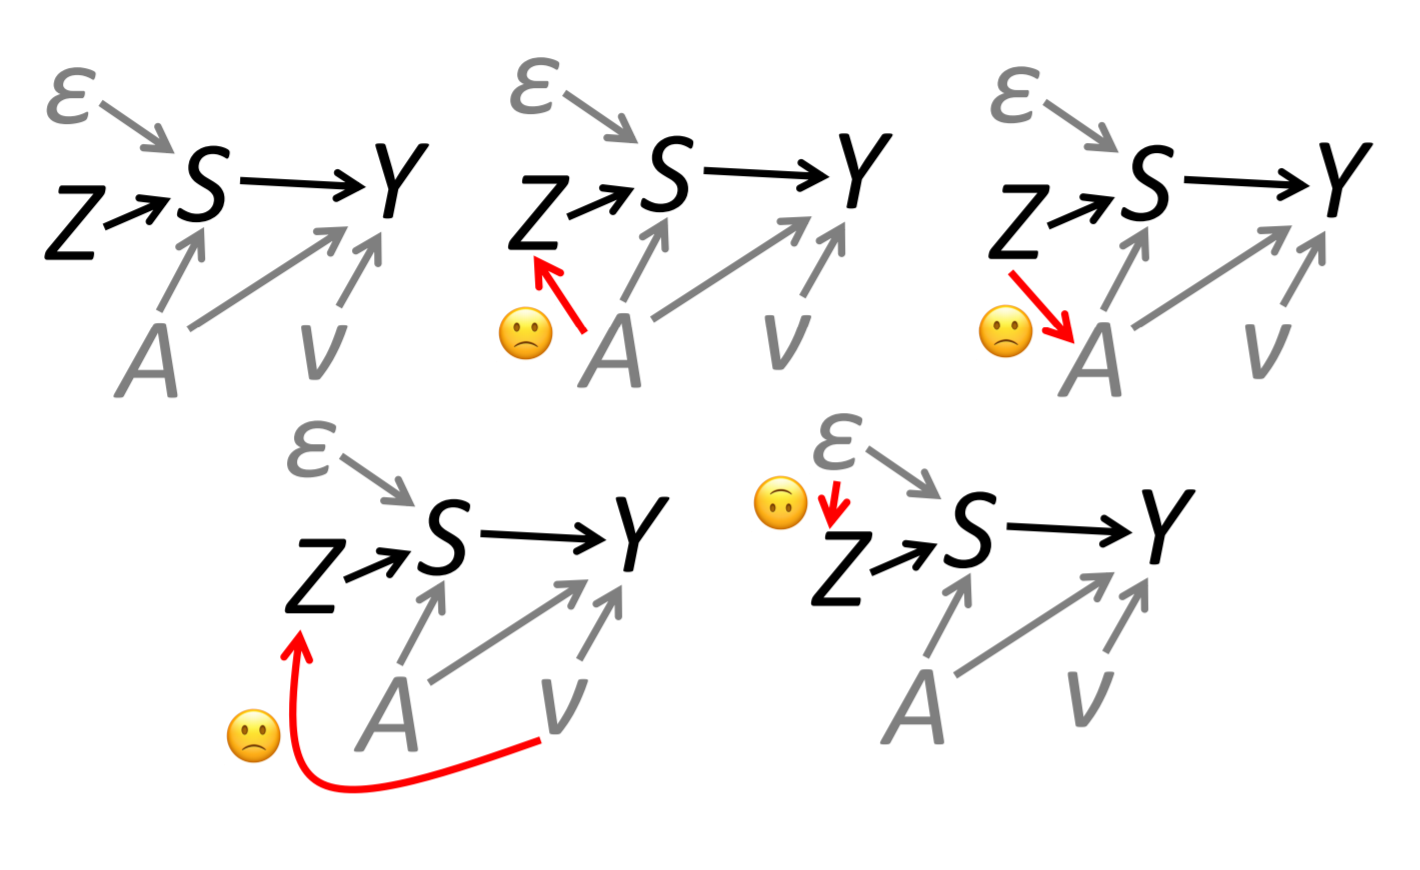
\includegraphics[width=0.5\linewidth]{images/iv-direct-graph.png}
    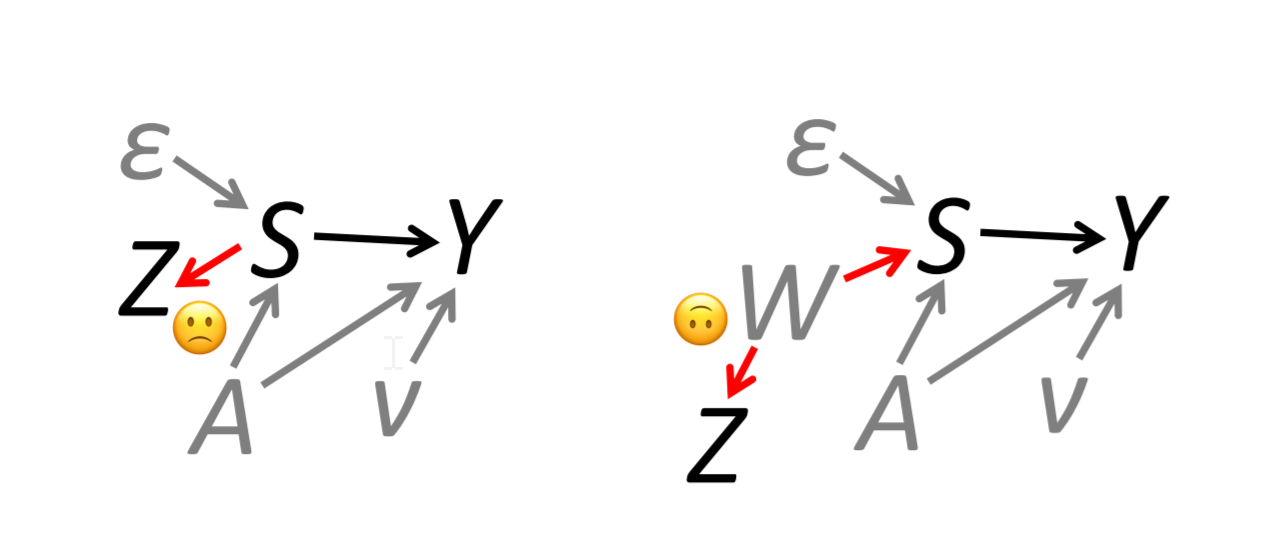
\includegraphics[width=0.5\linewidth]{images/iv-direct-figure2.png}
\end{figure}
The last case is especially interesting.
Notice that in the last case we should \textit{not} control over $\varepsilon$ because that is a collider. Also the one with $W$ as collider.
So it actually does not matter how $z$ and $s$ are correlated, $z$ does \textit{not} have to have causal effect on $s$. 


\textbf{Wald Statistic}

If the IV $z_i$ is a binary variable, then 2SLS is Wald statistic.
For Wald statistic:
\[
    \rho = \frac{E[y_i | z_i =1] - E[y_i | z_i=0]}
    {E[s_i | z_i =1] - E[s_i|z_i=0]}
\]
The intuition is straightforward,
since the only channel for $z_i$ to influence $y_i$ is through $s_i$.


\textbf{GMM Framework}

We can also do IV in GMM framework.
The benefit of using GMM is to have variance correct.
\[
    E [Z(Y - \beta X)] = 0
\]


\chapter{Diff in Diff} % (fold)
\label{cha:diff_in_diff}

The Diff-in-Diff estimators family include:
\begin{itemize}
    \item Plain diff-in-diff
    \item Synthetic control. See \citet{AbadieDiamondHainmueller2010}, \citet{Xu2017}
\end{itemize}


\chapter{Network Effect}
\label{cha:network_effect}

Network in Migration:
\begin{itemize}
    \item \citet{BayerRossTopa2008} leverages two effects: 1) the network effect is very local (say block); 2) the matching of unobservables happen at a larger neighborhood level. Then the migration difference of blocks within the same group can be attributed to network effects.
    \item \citet{StuartTaylor2019,StuartTaylor2019a}. They propose a new index to measure network effects, using individual level migration data.
\end{itemize}

\section{Bayer, Ross, Topa, 2008 JPE} % (fold)
\label{sec:bayer_ross_topa_2008_jpe}

\textbf{\fullcite{BayerRossTopa2008}}

This paper is the first one that uses the geographic in local areas to identify the network effects.
The identification assumption of their paper is:
\begin{enumerate}
    \item The network effect is very local (say block level);
    \item The matching of unobservables happen at a larger neighborhood level (say Census block group level)
\end{enumerate}

Their baseline regression is:
\[
    W_{i j}^{b}=\rho_{g}+\alpha_{0} R_{i j}^{b}+\varepsilon_{i j}
\]
where $i,j$ are two different individuals, $W_{ij}^b$ is a dummy which equals 1 if $i,j$ works in the same block; 
$R_{ij}^b$ equals 1 if they reside in the same block; 
$\rho_g$ is the fixed effect at block level.
The parameter of interest is $\alpha_0$ 

% section bayer_ross_topa_2008_jpe (end)



\section{Stuart, Taylor, 2019 (wp)} % (fold)
\label{sec:stuart_taylor_2019_wp}

\textbf{\fullcite{StuartTaylor2019}}


The basic idea of this paper is to use a diff-in-diff style estimator.
Pick two similar born towns $j$ and $j'$, which should have similar ex-ante migration probability to another town $k$.
Then the observed migration difference $D_{jk}$ and $D_{jk'}$ is explained by the network effect. 
They propose a simple index to capture the network effect, and they allow the network effect to differ across the destination towns.

The baseline regression is: (modified from \cite{BayerRossTopa2008})
\[
    D_{i, j(i), k} D_{i^{\prime}, j\left(i^{\prime}\right), k}=\alpha_{g, k}+\sum_{j \in g} \beta_{j, k} 1\left[j(i)=j\left(i^{\prime}\right)=j\right]+\epsilon_{i, i^{\prime}, k}
\]
where $j$ is the birth town of $i$, $k$ is the destination, $D_{i,j,k}$ is a dummy which equals 1 if $i$ moves from $j$ to $k$; $g$ is a group of towns where it is assumed that the ex-ante moving probability within the same group is the same.
the parameter of interest is $\beta_{j,k}$.
They show the following things:
\begin{enumerate}
    \item $\beta_{j,k} = C_{j,k}$, where $C_{j, k} \equiv \sum_{i \neq i^{\prime} \in j} \operatorname{Cov}\left[D_{i, j, k}, D_{i^{\prime}, j, k}\right] /\left(N_{j}\left(N_{j}-1\right)\right)$ being the average covariance of the location decisions for two migrants from the same town;
    \item $\alpha_{g,k} = P^2_{g,k}$, where $P_{j, k} \equiv \mathbb{E}\left[D_{i, j, k}\right]$ is the \textit{ex-ante} probability of an individual migrating from $j$ to $k$.
\end{enumerate}
Their main argument: $\beta_{j,k}$ does not well capture the network effect, because it varies with ex-ante moving probability $P_{j,k}$:
\[
    \beta_{j,k} = C_{j,k} = P_{g,k}(\mu_{j,k} - P_{g,k})
\]
where $\mu_{j, k} \equiv \mathbb{E}\left[D_{i, j, k} | D_{i^{\prime}, j, k}=1\right]$.


To overcome this problem, they propose a intuitive network index $\Delta_{j,k}$, which captures the expected increase in the number of people from birth town $j$ that move to destination $k$:
\[
    \Delta_{j, k} \equiv \mathbb{E}\left[N_{-i, j, k} | D_{i, j, k}=1\right]-\mathbb{E}\left[N_{-i, j, k} | D_{i, j, k}=0\right]
\]
they show that $\Delta_{j,k}$ can be derived from observable moving patterns:
\[
    \Delta_{j, k}=\frac{\left(\mu_{j, k}-P_{g, k}\right)\left(N_{j}-1\right)}{1-P_{g, k}}=\frac{C_{j, k}\left(N_{j}-1\right)}{P_{g, k}-P_{g, k}^{2}}
\]

% section stuart_taylor_2019_ (end)


% chapter diff_in_diff (end)



\part{IO} % (fold)
\label{prt:io}


\chapter{Demand Estimation} % (fold)
\label{cha:demand_estimation}

Basics: \citet{BerryLevinsohnPakes1995}

Micro moments: \citet{Petrin2002}, \citet{BerryLevinsohnPakes2004}

Vertical relationships: \citet{Villas-Boas2007}, \citet{CrawfordYurukoglu2012}

Durable consumptions: \citet{HendelNevo2006}


\chapter{Vertical Relationships} % (fold)
\label{cha:vertical_relationships}

\paragraph{\citet{CrawfordYurukoglu2012}} This paper uses a Nash-in-Nash model to model the bargain process between upstream and downstream firms.
Recall that in \citet{Villas-Boas2007}, the contract is either linear, or that upstream/downstream has all bargain power. This paper is a generalization in this aspect.


% chapter vertical_relationships (end)

\section{Villas-Boas, 2007 RES} % (fold)
\label{sec:villas_boas_2007_res}

\textbf{\fullcite{Villas-Boas2007}}

The main goal of this paper is to recover the margins of both retailers and wholesalers with only retailing data.
Unlike later papers like \citet{CrawfordYurukoglu2012} which endogenizes a bargain process, the relationship between the upstream and downstream firms are assumed to be one of the several stylized forms: simple linear contract, wholesaler with all rents, retailer with all rents.
The paper tries to tell which one is more likely to be the truth among these stylized models.


The demand side is typical BLP with random coefficients $\alpha_i, \beta_i$:
\[
    U_{i j t}=d_{j}+d_{t}+x_{j t} \beta_{i}-\alpha_{i} p_{j t}+\xi_{j t}+\epsilon_{i j t} \tag{1}
\]

The paper focuses on the vertical structural of the supply side.

\paragraph{Scenario 1: simple linear pricing model}

The retailer profit function is:
\[
    \pi_{r t}=\sum_{j \in S_{r t}}\left[p_{j t}-p_{j t}^{w}-c_{j t}^{r}\right] s_{j t}(p)
\]
and we can write FOC for product $j$ of retailer $r$:
\[
    s_{j t}+\sum_{m \in S_{r t}}\left[p_{m t}-p_{m t}^{w}-c_{m t}^{r}\right] \frac{\partial s_{m t}}{\partial p_{j t}}=0 \quad \forall j \epsilon S_{r t}, \quad \text { for } r=1, \ldots, N_{r}
    \tag{5}
\]
which is equivalent to the following equation holds for all commodities in the market $\mathcal J$:
\[
    s_{it} + \sum_{j \ in \  \mathcal J_t} [p_{jt} - p^w_{jt} - c^r_{jt}] \mathds 1\{i,j \in \mathcal J_r\} \frac{\partial s_{jt}}{ \partial p_{it}} = 0,\ \  \forall i \in \mathcal J_t, \forall t
\]

Then stack all products in the market together in the market to write the matrix form:
\begin{align*}
    s_t(p) + (T_r * \Delta_r)(p_t-p_t^w-c_t^w) = 0 \\
    \Rightarrow
    p_{t}-p_{t}^{w}-c_{t}^{r}=-\left(T_{r} * \Delta_{r t}\right)^{-1} s_{t}(p)
    \tag{6}
\end{align*}
where $T_r$ is the ownership matrix, $T_r(i,j)$ equals to 1 if $i,j$ belong to the same owner, other wise 0. 
$\Delta_{rt}$ is the retailer's response matrix, $\Delta_{rt}(i,j)= \frac{\partial s_{jt}}{\partial p_{it}}$.
Both $p^w_t$ and $c^r_t$ are unobservable, other parts are observable. 
$\Delta_{rt}$ is estimated from the demand side.

Similarly, for wholesaler we have:
\[
    \pi_{w t}=\sum_{j \in S_{w t}}\left[p_{j t}^{w}-c_{j t}^{w}\right] s_{j t}\left(p\left(p^{w}\right)\right)
\]
the corresponding FOC is:
\[
    s_{j t}+\sum_{m \in S_{w t}}\left[p_{m t}^{w}-c_{m t}^{w}\right] \frac{\partial s_{m t}}{\partial p_{j t}^{w}}=0 \quad \forall j \epsilon S_{w t}, \quad \text { for } w=1, \ldots, N_{w}
\]

The $\frac{\partial s_{m t}}{\partial p_{j t}^{w}}$ for wholesalers are very complicated, because the wholesale price change in one product will induce all retailers to re-optimize their products.
Let $\Delta_{wt}(i,j)$ be $\frac{\partial s_{m t}}{\partial p_{j t}^{w}}$.
First notice that $\Delta_{wt} = \Delta_{pt}'\Delta_{rt}$, where $\Delta_{pt}$ is the derivative matrix of retail price to wholesale price. 
So the key for wholesaler FOC is to find $\Delta_{pt}$.
To obtain this, do total differentiation for all retail prices $dp_k,k=1,\ldots,N$ with respect to a wholesale price $p^w_f$ in the optimization equation (5) of retailers:
\[
    \sum_{k=1}^{N} \underbrace{\left[\frac{\partial s_{j}}{\partial p_{k}}+\sum_{i=1}^{N}\left(T_{r}(i, j) \frac{\partial^{2} s_{i}}{\partial p_{j} \partial p_{k}}\left(p_{i}-p_{i}^{w}-c_{i}^{r}\right)\right)+T_{r}(k, j) \frac{\partial s_{k}}{\partial p_{j}}\right]}_{g(j, k)} d p_{k} - 
    \underbrace{T_{r}(f, j) \frac{\partial S_{f}}{\partial p_{j}}}_{h(j, f)} d p_{f}^{w}=0
\]
Stack all products together, we have:
\[
    \frac{d p}{d p_{f}^{w}}=G^{-1} H_{f}
\]
where $G,H$ are matrixes for $g,h$ respectively.
Thus the FOC of wholesalers can be written as:
\[
    p_{t}^{w}-c_{t}^{w}=-\left(T_{w} * \Delta_{w t}\right)^{-1} s_{t}(p)
    \tag{11}
\]

\paragraph{Estimation}

This paper does not really estimate the supply side.
Instead, it estimates only the demand side of retailers, then use this demand side to back out the margins of both retailers and wholesalers.
The margins can be backed out by equation (6) and (11) RHS.



% section villas_boas_2007_res (end)

\chapter{Dynamic Estimation}
\label{cha:dynamic_estimation}

\citet{Rust1987} proposes Nested Fixed Point approach.
The bad thing is computation complexity.

\section{Hendel, Nevo, 2006 EMCA} % (fold)
\label{sec:hendel_nevo_2006_emca}

\textbf{\fullcite{HendelNevo2006}}

This paper estimates a model with consumer storage. 
They solved two problems: 
1) the inventory (a state variable) is unobservable to researchers;
2) the state space is too large.

A key feature of their model is that they can separate a static problem from the dynamic problem, and use that static problem to estimate the purchasing utility parameters, which includes the brand heterogeneity.
The dynamic problem is then independent of brand, but solely quantity related.

\paragraph{Model}

The flow utility is assumed to be:
\[
    u\left(c_{h t}, \nu_{h t} ; 
    \boldsymbol{\theta}_{h}\right)+\boldsymbol{\alpha}_{h} m_{h t}
\]
where $c_{ht}$ is the quantity consumed (not purchased) by consumer $h$ in time $t$; 
$m_{ht}$ is the consumption of the outside good.
Note that $c_{ht}$ is assumed to be the total consumption of all brands: 
$c_{ht} \equiv \sum_{j} c_{jht}$. 
This implies: 
1) the consumption has no brand preference;
2) the consumption will not be affected by which brand is at storage.

Then we can write the dynamic problem:
\begin{align*}
    V\left(s_{1}\right)
    &{=\max _{\left\{c_{h}\left(s_{t}\right), d_{h j}\left(s_{t}\right)\right\}} \sum_{t=1}^{\infty} \delta^{t-1} E[u\left(c_{h t}, \nu_{h t} ; \boldsymbol{\theta}_{h}\right)-C_{h}\left(i_{h, t+1} ; \boldsymbol{\theta}_{h}\right)}\\
    & +\sum_{j} d_{h j x t}\left(\alpha_{h} p_{j x t}+\xi_{h j x}+\beta_{h} a_{j x t}+\varepsilon_{h j x t}\right) | s_{1}]
\end{align*}
\[
    \begin{array}{ll}{\text { s.t. } \quad 0 \leq i_{h t}, \quad 0 \leq c_{h t},} & {0 \leq x_{h t}, \quad \sum_{j, x} d_{h j x t}=1} \\ {} & {i_{h, t+1}=i_{h t}+x_{h t}-c_{h t}}\end{array}
\]
where $i_{ht}$ is the inventory of consumer $h$ at time $t$; 
$d_{hjxt}$ equals 1 if brand $j$ and size $x$ is purchased;
$C_h$ is the storage cost;
$a_{jht}$ is the advertising variable.

Notice, the purchasing per se (in addition to the following consumption) has utility here, which I do not understand.
Also, the product differentiation takes place at \textit{purchase}, not \textit{consumption}.
As mentioned by the authors, this assumption ``helps reduce the state space. Instead of the whole vector of brand inventories, only the total quantity in stock matters, regardless of brand.''

\paragraph{Estimation}

The estimation process of this dynamic problem is not trivial.
First, the state variable inventory $i_t$ is not observable.
Second, the state space include brand, variety, price and advertisements, which is very large and intractable.

To solve the unobservable inventory problem, they use the fact that the optimal consumption can be calculated. 
For this moment assume that the inventory $i_t$ is observable, then the researcher can derive the optimal consumption $c_t$ since all state variable now observable.
Then the researcher can derive the purchasing probability $d_{t+1}$ which is observed in the data, and, therefore, derive $i_{t+1}$.
The probability of the observed sequence of purchases is:
\[
    \begin{array}{l}{\operatorname{Pr}\left(d_{1} \cdots d_{T} | p_{1} \cdots p_{T}\right)} \\ {\quad=\int \prod_{t=1}^{T} \operatorname{Pr}\left(d_{t} | p_{t}, i_{t}\left(d_{t-1}, \ldots, d_{1},\right.\right.} \\ 
    \quad \quad \quad \quad \quad \quad {\left.\left.\nu_{t-1}, \ldots, \nu_{1}, i_{1}\right), \nu_{t}\right) d F\left(\nu_{1}, \ldots, \nu_{T}\right) d F\left(i_{1}\right)}\end{array}
\]
where $F(i_1)$ is observed in the data.

\paragraph{Dimension Reduction}

The dimension is too high for practical estimation.
So the paper uses \textit{inclusive value} to reduce the dimension. 
The steps are as following:
\begin{enumerate}
    \item Estimate the static parameters, which are purchasing utility parameters;
    \item Simplify the state of DP using inclusive value;
    \item Use nested fixed point to estimated the simplified DP problem.
\end{enumerate}

Recall that the consumption utility does not depend on the brand but only on the quantity; then it is natural that the optimal consumption depend only on the quantity of storage, independent of the brand. (details see their lemma 1)
This is an important assumption for them to separate the consumption and the purchasing. 
Then it's convenient to define:
\[
    M\left(s_{t}, j, x\right)
    \equiv \operatorname{Max}_{c}\left\{u\left(c+\nu_{t}\right)-C\left(i_{t+1}\right)+\delta E\left(V\left(s_{t+1}\right) | d_{j x}, c, s_{t}\right)\right\}
\]
The above paragraph is saying that, conditional on quantity $x$, $M(s_t,j,x)=M(s_t,j',x)$.
Then it's direct to show that:
\[
  \begin{aligned} \operatorname{Pr}\left(d_{j t}=1 | x_{t}, i_{t}, p_{t}, \nu_{t}\right) &=\frac{\exp \left(\alpha p_{j x t}+\xi_{k x}+\beta a_{k x t}\right)}{\sum_{k} \exp \left(\alpha p_{k x t}+\xi_{k x}+\beta a_{k x t}\right)} \\ &=\operatorname{Pr}\left(d_{j t}=1 | x_{t}, p_{t}\right) \end{aligned}  
\]
Using conditional probability rule, we can rewrite the joint choice probability of $j$ and $x$ to be:
\begin{align*}
\operatorname{Pr}\left(d_{j t}=1, x_{t} | p_{t}, i_{t}, \nu_{t}\right)&=
\operatorname{Pr}\left(d_{j t}=1 | p_{t}, x_{t}, i_{t}, \nu_{t}\right) 
\operatorname{Pr}\left(x_{t} | p_{t}, i_{t}, \nu_{t}\right) \\
&= \operatorname{Pr}\left(d_{j t}=1 | x_{t}, p_{t}\right) 
\operatorname{Pr}\left(d_{j t}=1 | p_{t}, x_{t}, i_{t}, \nu_{t}\right) 
\end{align*}
In the first step, we estimate the first part separately, which give us purchasing utility parameters.

Then in the second step, we show that the DP problem can be simplified using the inclusive value.
The inclusive value $\omega_{xt}$ is defined as:
\[
    \omega_{x t}=\log \left\{\sum_{k} \exp \left(\alpha p_{k x t}+\xi_{k x}+\beta a_{k x t}\right)\right\}
\]
Notice that the $\omega_{xt}$ is known up to parameters which can be estimated in the first step.
This simplifies the DP problem because $\omega_{xt}$ is a scalar, so we do not have to track the price distribution for different brands.
So if we can rewrite the DP using $\omega_{xt}$, we solve the problem of 
It can be shown that the DP problem is equivalent to the below DP using the inclusive value: (see their appendix for proof)
\[
    \begin{array}{l}{V\left(i_{t}, \omega_{t}, \varepsilon_{t}, \nu_{t}\right)} \\ {\quad=\operatorname{Max}_{\{c, x\}}\left\{u\left(c+\nu_{t}\right)-C\left(i_{t+1}\right)+\blue{\omega_{x t}}+\varepsilon_{x t}\right.} \\ 
    \quad \quad \quad {\left.\quad+\delta E\left[V\left(i_{t+1}, \blue{\omega_{t+1}}, \varepsilon_{t+1}, \nu_{t+1}\right) | i_{t}, \omega_{t}, \varepsilon_{t}, \nu_{t}, c, x\right]\right\}}\end{array}
\]
The key of the proof is to use the fact that all error terms are i.i.d. and T1EV distributed, so there is a closed form of expected maximum utility over alternative brands, which is $\omega_{xt}$.

With this, we can calculate the probability of a particular purchasing sequence using previous chain method.

% section hendel_nevo_2006_emca (end)



% chapter demand_estimation (end)

\chapter{Observational Learning} % (fold)
\label{cha:observational_learning}

Empirical Observational Learning:
\begin{itemize}
    \item Literature Review: \textcite{Sorensen2017}
    \item IO: \textcite{Moretti2011}, \textcite{HendricksSorensenWiseman2012}, \textcite{Newberry2016}, \textcite{LiWu2019}, \textcite{HollenbeckMoorthyProserpio2019}
    \item Development: \textcite{BobonisFinan2009}, \textcite*{AngelucciDeGiorgiRangelEtAl2010}, \textcite*{BursztynEdererFermanEtAl2014}
\end{itemize}

The \textit{observational learning} is often frequently associated with \textit{peer effects}.
Observational learning can be seen as a mechanism underlying peer effect \citep{BursztynEdererFermanEtAl2014}.

% chapter observational_learning (end)


\part{Education}

\chapter{School Effectiveness (Value Added)}

Notice that most structural paper makes the school value added as homogeneous within a school, not heterogeneous across students, why? 
Examples include \citet{Allende2019,Neilson2018}.
This can be another contribution of my paper.



\section{Black-White Gap} % (fold)
\label{sec:black_white_gap}

\paragraph{\citet[AEJ:AE]{ElderZhou2020}} This paper shows that the black-white gap in non-cognitive ability is underestimated. 
Because non-cognitive ability is reported by the teachers, and the teacher will use similar peers as references. 
Black students have poorer behaved peers than their white classmates.
The authors use more objective measures like test scores to correct this subjective measure.
The underlying assumption is that there are correlations between the objective and subjective measures between schools.
This paper needs further read, I have not read the actual method yet.

% section black_white_gap (end)



% chapter end


\chapter{Demand for Education}

A huge literature in school choice:
\begin{itemize}
    \item Theory paper: \textcite{BarseghyanClarkCoate2019}
    \item Empirical paper: \citet{HastingsKaneStaiger2009}, \citet*{DemingHastingsKaneEtAl2014}, \citet*{BurgessGreavesVignolesEtAl2015}, \textcite{Walters2018}
    \item Combine with location choice:   
    \begin{itemize}
        \item Methodology paper combining residential sorting with school choice: \textcite{Rothstein2006}, \textcite{BayerTimmins2007}, \textcite{BayerFerreiraMcMillan2007}, \textcite{BayerMcMillan2010}, \Textcite{BayerMcMillanMurphyEtAl2016}
        \item Empirical: \textcite{CordesSchwartzStiefel2019} uses NYC residential data to study the effect of mobility; \citet{EppleJhaSieg2018} seems to also estimate a demand model with student sorting
    \end{itemize}
    \item Using discrete choice models: \citet{Allende2019}, \citet{Neilson2018}
\end{itemize}

Some other papers focus more on the school competition:
\begin{itemize}
    \item Reduced form: \textcite{Lavy2010} uses DiD and border discontinuity to show that the school competition in Tel-Aviv has positive results.
\end{itemize}

There are certain reasons why the competition among schools will not work.
\begin{enumerate}
    \item Schools (principals and teachers) may lack the incentive to correspond to the competition
    \item Schools may lack the flexibility to change. E.g. they cannot fire under-qualified teachers at their own discretion.
    \item Families may lack incentive to correspond to the ``value added'' of schools, but simply prefer schools with better peers \parencite{AbdulkadirogluPathakSchellenberg2017,MacLeodUrquiola2015,MacLeodUrquiola2019}.
    \item Families may not be able to identify effective schools \parencite{AllendeGallegoNeilson2018}
\end{enumerate}


Heterogeneous student response to inputs:
\begin{itemize}
    \item \textcite{Bau2019} shows that rich students are more responsive to quality.
    \item \textcite{JacksonJohnsonPersico2016} shows that school inputs are more valuable to poor students (p.192)
\end{itemize}


Endogenous school differentiation:
\begin{itemize}
    \item \textcite{MacLeodUrquiola2012}, \textcite{GilrainePetronijevicSingleton2019}
    \item \citet{Neilson2018}
\end{itemize}



\subsection*{Review: Demand for schools}

\paragraph{\citet{HastingsKaneStaiger2009}}
They use a simple exploded logit model to show that the demand for high academic quality are heterogeneous across families.
The more affluent families put higher weights on academic performance, but poorer families and minorities put higher weights in the race composition of the school.

Cons:
\vspace{-1em}
\begin{enumerate}
    \item In their utility function (4), they directly include school average test score $S_j$, which is obviously endogenous of student composition. They do not deal with this using IV.
    \item They do not have an unobserved attractiveness term $\xi_j$ as BLP in the utility.
\end{enumerate}

\paragraph{\citet{EppleJhaSieg2018}}

The main contribution of this paper is that they incorporate the peer effects into demand estimation. 
They also deal with the limited capacity problem by introducing a \textit{shadow price} for over-subscribed schools.
Note that this is actually tricky, because when they estimate the demand, they assume no capacity constraint, and the constraint only holds in computing the counterfactual equilibrium.

The main contribution of their paper is an algorithm of calculating the counterfactual equilibrium with peer effects.
The demand estimation part is quite standard.
They use MLE for the demand estimation.

\red{Add their IV strategy}

Cons:
\begin{enumerate}
    \item The demand estimation does not consider the capacity constraint
    \item The location sorting is not considered in the model
\end{enumerate}


\section{Review: School Competition} % (fold)
\label{sec:review_spillover_effects}

\subsection*{Charter School Spillover Effects}

\paragraph{\citet*{BookerGilpatricGronbergEtAl2008}} 

This paper uses a longitudinal data in Texas to show that charter schools in Texas have positive spillovers in nearby TPS.
They use panel data to control student/campus fixed effect to exclude the sorting effect.
They focus on the response at district level instead of campus level.
One charter school nearby increase the Math and Reading test score by 0.021 sd; as a comparison, those who move to another campus have a negative effect of 0.104 sd on Math. 
They also find the effect is more salient for black and Hispanic students.


\section{Discrete School Choice} % (fold)
\label{sec:discrete school choice}

There are a growing literature showing this, borrowing tools from IO, including \citet{Neilson2018}, \citet{Allende2019}.

\paragraph{\citet[JMP]{Allende2019}}

This paper features \underline{endogenous school quality} + \underline{student sorting} + \underline{social interactions}.
\grey{Worth carefully re-reading, and also the reference here.}

The schools have three stages: 1) quality investment; 2) price setting; 3) school demand based on quality, price, and social interactions.

The school quality $\theta_{jt}$ is assumed to be \underline{uniform} within a school, though it can depend on certain policies:
\[
    Y_{i j t}(\tau)=\mathbf{X}_{i t}^{\prime} \pi^{x}+\theta_{j t}(\tau)+\epsilon_{i j t}
\]
The school quality $\theta_{jt}$ can be further decomposed to inputs:
\[
    \theta_{j t}(\tau)=\mathbf{z}_{j t}(\tau)^{\prime} \pi^{z}+\underbrace{\mathbf{I}_{\mathrm{jt}}(\tau)^{\prime} \pi^{I}(\tau)+\epsilon_{j t}^{s}(\tau)}_{\mu_{j t}(\tau)}
\]
Notice, in this paper \blue{only $\mu_{jt}(\tau)$ is relevant}, there is no further decomposition of the terms.

\mysubtitle{Demand side:}

Individual utility is typical as in BLP and \citet{Neilson2018}. It also includes some unknown student level unobservables, I guess this is because they do not have huge computation burden in other parts.

\grey{Why the price coefficient $\alpha_i$ and distance coefficient $\beta_i^d$ not have unobservable part? What is special about price and distance? (page 20)}

The demand is based on \textit{nodes} and \textit{schools}. 
This setting is similar to \citet{Neilson2018} and leverages the detailed node-level geographic data.
The choice probability is defined as:
\[
    \mathcal{S}_{i j t}^{n k}\left(\boldsymbol{\mu}, \mathbf{p}, \mathbf{z}^{y}, \mathbf{z}^{e}\right)=\left(\frac{\exp \left(U_{i j t}\left(\boldsymbol{\mu}, \mathbf{p}, \mathbf{z}^{y}, \mathbf{z}^{e}\right)\right)}{\sum_{l \in \Omega_{i}} \exp \left(U_{i l t}\left(\boldsymbol{\mu}, \mathbf{p}, \mathbf{z}^{y}, \mathbf{z}^{e}\right)\right)}\right)
\]
where $i$ is student, $j$ is school, $t$ is time, $n$ is node, $k$ is the student type. 
Student type $k$ is observable. $\mu$ is school quality, $p$ is tuition, $z^y, z^e$ are school observable characteristics.
Note that the information is aggregated at the node-school level, so she uses GMM instead of MLE, thus the computation burden is smaller.

Student body composition is assumed to be perfectly expected by the family.

\mysubtitle{Supply side:}

Similar as in \citet{Neilson2018}, the private schools are profit-maximizing, with following cost structure:
\[
    M C_{j}\left(\mu_{j t}\right)=\sum_{l} \gamma_{l} w_{j t}^{l}+\gamma_{\mu} \mu_{j t}+\omega_{j t}
\]
\[
    F C_{j}\left(\mu_{j t}\right)=\sum_{l} \lambda_{l} w_{j t}^{l}+\psi_{j t} \mu_{j t}, \quad \text { where } \psi_{j t}=\bar{\psi}_{j}+\Delta \psi_{j t}
\]
\grey{One difficulty in my paper is that I cannot really observe the cost characteristics $w_{jt}^l$, but instead the monetary expenditure. Possible solutions: to find more direct cost characteristics data.}

A worth learning feature in this paper is that Allende \blue{(analytically) decompose the effects} to direct effects, peer effects, and strategic social effects, which makes it clear about the channel of this model.

\mysubtitle{Identification}

There are three endogeneity to be solved: the quality of school, the price of school, and the student composition.

The main identification leverages a natural experiment: the public school teacher strike in Lima. This makes more students turn to private schools.

IV for \underline{student body composition}:
\begin{itemize}
    \item Lagged strike exposure index
    \item Local market structure: share of private and number of schools
    \item Local demographics: share of high SES
\end{itemize}

IV for \underline{price and quality}: (all distance weighted when applicable)
\begin{itemize}
    \item Public school teacher wage index
    \item Public school teacher vacancies for post-reform contracts (distance weighted)
    \item Stock of graduates with education degrees ($t-1$)
    \item Tests scores for teachers ($t-1$)
    \item The flow of new graduates with education degrees in the market
\end{itemize}

Notice that she presents all the first stages to show relevance.
\grey{Seems this only requires school level data so can be done soon?}

RD to identify \underline{price parameters}:
\begin{itemize}
    \item There is individual level variation in price generated discontinuity of private school voucher program.
\end{itemize}

% section endogenous_school_decisions (end)


% section review_spillover_effects (end)



\section{Bayer, Timmins, 2007 EJ} % (fold)
\label{sec:bayer_timmins_2007_ej}

\textbf{\fullcite{BayerTimmins2007}}

This paper proposes a way to estimate the local spillover effects (summarized by the share of people living in location $j$, $\sigma_j$).
The basic idea is to use the BLP framework, but have $\sigma_j$ in the utility function.
They show that there is no need to exactly solve the model, and the complication mainly comes from multi-equilibria phenomena which they solve by proposing a semi-likelihood estimator as in BBL.
They do not encompass the followings in the paper: the endogenous price, the school choice problem. But both should be not difficult to deal with.

The utility is:
\begin{align}
    U_{i, j}=\mathbf{X}_{j}^{\prime} \boldsymbol{\beta}_{i}+\alpha_{i} \sigma_{j}+\xi_{j}+\varepsilon_{i, j}
\end{align}
Note:
\begin{itemize}
    \item $\sigma_j$ is share of individuals who choose location $j$. This is definitely endogenous since it's determined in the equilibrium, and needs to be instrumented.
    \item There is no price included in above utility. If included, needs additional instrument for price.
    \item Other parts are standard BLP
\end{itemize}

\textbf{Equilibrium:}

Given $\sigma,\xi$ (both being vector), the individual choice probability is:
\[
    P_{i, j}=g_{i, j}\left(\mathbf{Z}_{i}, \mathbf{X}, \boldsymbol{\sigma}, \xi\right) \forall i, j
\]
where we have the closed from for $g(\cdot)$ if $\varepsilon_{i,j}$ follows i.i.d. T1EV.

Aggregate over individuals and we get the shares:
\[
    \sigma_{j}=\int g_{i, j}\left(\mathbf{Z}_{i}, \mathbf{X}, \boldsymbol{\sigma}, \xi\right) \mathrm{d} h(\boldsymbol{Z}) \forall j
\]
where $h(Z)$ is the density of $Z$ in the population, which is known. 
KZ: notice that we can use Nevo strategy if we can observe individual level demographics.

Then the above two equations define the equilibrium. 
The uniqueness is not guaranteed in general, unless the local spillover effects $\alpha_i$ are constrained to be negative.
See \textcite{BayerMcMillan2010} for more details on uniqueness conditions.

\textbf{Estimation:}

Sketch:
\begin{itemize}
    \item The estimation is basically BLP, but we need to find instruments for market shares $\sigma_j$. The two steps approach below is very similar to that in \citet{Hackmann2019}.
    \item The equilibrium may have multiple equilibria, needs to be dealt with. The authors pick an equilibrium selection rule $P(\sigma | \Omega)$ and non-parametrically estimate this probability along with the likelihood. But other more robust approach may be used as well, like the moment inequality in \citet{CilibertoTamer2009}.
    \item Step 1: Estimate $\delta_j$ as fixed effects, as well as $\beta_1, \alpha_1$
    \item Step 2: Estimate the mean utility parameters within $\delta_j$
\end{itemize}

First rewrite the utility function to be the addition of mean utility $\delta_j$ and idiosyncratic utility part:
\[
    U_{i, j}=\delta_{j}+\mathbf{X}_{j}^{\prime} \mathbf{Z}_{i} \boldsymbol{\beta}_{1}+\sigma_{j} \mathbf{Z}_{i} \boldsymbol{\alpha}_{1}+\varepsilon_{i, j}
\]
where
\[
    \delta_{j}=\mathbf{X}_{j}^{\prime} \boldsymbol{\beta}_{0}+\alpha_{0} \sigma_{j}+\xi_{j}
\]

Since the possibility of multiple equilibria, the likelihood is not well defined. 
The authors then define $P(\sigma | \Omega)$ as the equilibrium selection rule, where $\Omega$ contains exogenous data $\{X,Z\}$ and parameters $\left\{\delta, \alpha_{1}, \beta_{1}, \Sigma\right\}$.
Importantly, $\Omega$ does not contain unobservable individual level shocks $\varepsilon_{ij}$.
\[
    L=P(\boldsymbol{\sigma} | \mathbf{\Omega}) \prod_{i} \prod_{j} P_{i}(j | \boldsymbol{\sigma}, \mathbf{\Omega})^{I_{i j}}
\]
Here, $P(\sigma | \Omega)$ does not need to be estimated! (see later); and for given $(\sigma, \Omega)$, the $P_i(j)$ can be calculated.
\blue{Importantly,} different from standard entry model in IO like \citet{CilibertoTamer2009}, here our equilibrium selection rule does not depend on unobservable terms $\varepsilon_{ij}$.
This relies on the assumption that for all observable $\{X,Z\}$, there are continuum number of consumers with different $\varepsilon_{ij}$.
This is similar to the incompelete information assumption made in \citet{Seim2006}.
Therefore, the likelihood of the two components are orthogonal to each other, and we can estimate the second part only, assuming that each individual behaves optimally in the \textit{observed} equilibrium.

\textbf{Instruments:}

\blue{The instruments are the most important contribution of this paper.}

In the first step MLE, where the mean utility $\delta_j$ is estimated as a fixed effect, we do not need IV.
But we use GMM to estimate the parameters within mean utility, then we need IV.
We need IV because $\sigma_j$ is correlated with $\xi_j$. So we need IV which is correlated with $\sigma_j$ but uncorrelated with $\xi_j$.

The IV chosen here are similar to BLP IV, they choose the fixed attributes of other (nearby) locations.
They further uses a function to summarize the impact of such fixed attributes to a single instrument of share.
``This corresponds to using the predicted share of individuals that chooses a location based only on the observed, exogenous choice and individual characteristics used in the model, ignoring the role of local spillovers. ''

For the identification to really work, one needs some choice set variations. 
For example, there are several markets and in each market the consumers will have different choice sets.
Their table 3 shows that IV approach performs poorly without choice set variation.

% section bayer_timmins_2007_ej (end)


\section{Bayer, McMillan, 2010 wp} % (fold)
\label{sec:bayer_mcmillan_2010_wp}

\textbf{\fullcite{BayerMcMillan2010}}

The main purpose of this paper is to investigate whether the schools will respond to the competition. 
\[
    T^{m}=X_{c}^{m} \gamma_{c}+X_{n}^{m} \gamma_{n}+\gamma_{E} E^{m}+\varepsilon^{m}
\]
where $T^m$ is the average test score for school $m$, $X_c$ for household characteristics, $X_n$ for neighborhood controls, $E^m$ is the slope for demand-quantity curve.
The parameter of interest is $\gamma_E$.
Assume that the only unobservable is the school and teacher effort.
Think of the two polarized cases:
1) the school only cares about its teaching quality;
2) the school is rent seeking.
If the school only cares about teaching quality, then the schools' production function shall not be related with the competition, but only related with the observables and we can control that. 
\red{This claim is tricky.}
But if the school is rent seeking, then the schools face the following trade-offs: raising quality (by raising effort) can make the school more attractive which is valuable, but the induced higher effort is also costly.
Whether increasing quality is worthwhile depends on the responsiveness of demand to quality, the $E^m$.

Since $E^m$ is not observed directly in the data, it needs to be estimated.
They use \texttt{housing price} as the proxy for demand and use \texttt{school average test scores} as proxy for quality, conditional on school and student characteristics.
\blue{KZ: notice this quality is ``net quality'', trying to capture the effort induced quality.}
In order to overcome the endogeneity, they construct a discrete choice model, simultaneously choosing schools and locations, using BLP and methods in \textcite{BayerFerreiraMcMillan2007}.
\blue{Learn this technique.}
Then they conduct the counterfactual by increasing the test score of school $m$ by 1 s.d., then re-estimate the model and see how much the housing price will increase.
The resulting change captures the responsiveness of demand to quality.



% section bayer_mcmillan_2010_wp (end)

\chapter{School Finance} % (fold)
\label{cha:school_finance}

\textcite{JacksonJohnsonPersico2016} uses the School Finance Reforms (SFR) as exogenous variations of funding levels across school districts.
They use this variation to conduct DiD to show that higher expenditure will improve the student performance.


\chapter{Road Construction Program}


\noindent
\textbf{Some Research Ideas}

\begin{enumerate}
    \item The price elasticity of the farmers before and after market access
\end{enumerate}


\paragraph{\citet{Aggarwal2018}}

This paper is very similar to \citet{AdukiaAsherNovosad2019,AsherNovosad2019,Shamdasani2019} in terms of topics.
It includes a lot of details of the rural road construction plan effects.

To sum up:
\begin{enumerate}[nosep]
    \item Enrollments: enrollments for children less than 14 years old increase, while for elder than 14 years old decrease.
    \item Employment: the decrease in enrollments in elder teenagers all goes to increase in work, for both boys and girls (table 7).
    \item Employment sector: The increase in employment does not go to agriculture sector, for both boys and girls (table 8). For boys, the highest increase is in construction sector, and for girls is in animal rearing sector.
    \item Employment Locations: For prime-age men (25-45) and girls, huge increase in urban works, smaller increase for boys, almost no increase for prime-age women (table 11).
    \item Food diversity increases.
    \item Fertilizer use increases.
\end{enumerate}




\paragraph{\citet{AdukiaAsherNovosad2019}}

This paper studies the effect of massive road construction plan on rural enrollments in India.
The prior is ambiguous in the direction of the effect.
On the one hand, the road makes villagers easier to go outside for a higher wage, which lowers the incentive to stay at school;
on the other hand, the road makes the diploma more worthy since the human capital can sell a better price outside of the village, which increases the incentive to stay at school.
\textbf{Method:}
This paper uses a RD method to get the causal effect.
They leverage the fact that the road construction is discontinuous at some village population level, like 1000. But other covariates are continuous around that threshold.
\textbf{Data:}
The data they use is the same as \citet{AsherNovosad2019}, which is now public.
\textbf{Conclusion:}
They find that the middle school enrollments significantly increase after the road construction.


\paragraph{\citet{Shamdasani2019}}

This paper shows the massive road construction program has \textbf{heterogeneous} effect on villages, depending on their proximity to the town. 
Villages far from the town are still not convenient to go to the town after road construction. 
Thus, the first order effect for such villages is that they experience large gains in agriculture through crop diversification, with effects operating through rural-to-rural labor market integration.
Such effects are huge, in the scale of 20\% to 50\%.
\textbf{Method:} DiD.

Closely related to \citet{AsherNovosad2019}.
But this paper seems to use some independent data, worth reading.

KZ: My derived idea from this is that the road construction has heterogeneous effects to the different villages, thus should have different effects on school enrolling decisions.
For example, if there is no working opportunity in the village for high school graduates even after the road construction, then they shall not have incentive to enroll into high school.
In contrast, if in near villages high school graduates can migrate into the town, then they will have higher incentive to enroll.
The opposite may arise, though, if the young workers are important.

\paragraph{\citet{Reis2020}}

This paper uses a dynamic model similar to \citet{AttanasioMeghirSantiago2011} to study the joint problem of girls' enrolling and mothers' working decisions.

I don't understand why this paper can be published in IER...

\paragraph{\citet[IZA WP]{NajeebMoraleLopez-Acevedo2020}}

This paper documents some important facts about female employment in south Asia.
They find that 
``(i) overall since 2001, women’s employment participation across South Asian countries has been low and broadly unchanged; (ii) the gender employment gap emerges more clearly in middle age brackets; (iii) rural female employment is higher than urban; (iv) agriculture is the economic sector accounting for the greatest share of female employment, although this is slowly changing in some countries, and; (v) women with mid-level education tend to have lower employment rates than those with both lower and higher education.''



\clearpage
\singlespacing
\printbibliography
% \setlength\bibsep{0pt}
% \renewcommand\refname{Reference}
% \bibliographystyle{chicago}
% \bibliography{/Users/mac/Dropbox/Academic_Writings/reference-mac.bib}
% \bibliography{C:/Users/Kaida/Dropbox/Academic_Writings/reference-win.bib}

\end{document}